\section{Scaling of Statistical Inference}\label{sec:results}
%
Using the \funcX{} configuration deployed on RIVER described in~\Cref{subsec:FaaS_analysis_facilities}, \funcX{} is able to receive posted JSON serializations of the \pyhf{} pallet containing the background workspace and signal patches downloaded from HEPData~\cite{ATLAS_SUSY_1Lbb_pallet}, start \funcX{} worker nodes, send patched workspaces to each worker, fit the workspace and return the results with a user wall time of under 3 minutes.
As this wall time includes data transfer to and from the user's machine and RIVER, and worker node orchestration time, the time required for inference alone is even smaller.
Example typical run output and performance can be seen in~\Cref{lst:funcX_demo_output}.
The timing results over multiple trials for Ref.~\cite{ATLAS_SUSY_1Lbb_pallet}, using \pyhf{}'s NumPy backend and SciPy optimizer, along with the results from additional analyses~\cite{SUSY-2018-09,SUSY-2018-04} that have openly published probability models as \pyhf{} pallets on HEPData~\cite{ATLAS_SUSY_SS3L_pallet,ATLAS_SUSY_staus_pallet}, are summarized in~\Cref{table:performance} and visualized in~\Cref{fig:timing_barplot_river} and compared to the fit time for all patches on a single node.
All code used in these studies is publicly available on GitHub at Ref.~\cite{study_code,study_code_zenodo_doi}.\\

As \funcX{} endpoints run as users on the resources they are deployed on, and do not have elevated privileges, the number of worker nodes available is not an endpoint configurable option and so is not reported in this work.
Endpoints will utilize available resources effectively and allocate jobs to any available workers given their configuration settings.
A typical way to parameterize the range of available workers that an endpoint can scale work out on is by the \funcX{} endpoint configuration variables \texttt{max\_blocks} and \texttt{nodes\_per\_block} that control the available compute blocks --- the basic unit of resources acquired from an execution provider (e.g. a Slurm scheduler).
\texttt{max\_blocks} controls the maximum number of blocks that can be active per \funcX{} executor and \texttt{nodes\_per\_block} controls the number of nodes requested per block~\cite{Parsl_paper}.
These configuration parameters determine for a given value (generally $1$) of \texttt{parallelism} --- the ratio of task execution capacity to the sum of running tasks and available tasks --- how \funcX{} provisions blocks and distributes work to nodes.
The results summarized in~\Cref{table:performance} use $\texttt{max\_blocks}=4$ and $\texttt{nodes\_per\_block}=1$.
\clearpage

\begin{table}[htpb]
\centering
\caption{Scaling performance on RIVER for analysis fits over 10 trials compared to a single RIVER node. The reported wall fit time is the mean wall fit time of the trials. The uncertainty on the mean wall time corresponds to the standard deviation of the wall fit times. The number of worker nodes used is approximate as per-run reporting is not available.}
\label{table:performance}
\begin{tabular}{@{}lrrrr@{}}
\toprule
                      Analysis & Patches & Workers & Wall time (sec) & Single node (sec) \\
\midrule
 Eur. Phys. J. C 80 (2020) 691 &     125 &      85 &   $156.2\pm9.5$ &              3842 \\
             JHEP 06 (2020) 46 &      76 &      85 &    $31.2\pm2.7$ &               114 \\
Phys. Rev. D 101 (2020) 032009 &      57 &      85 &    $57.4\pm5.2$ &               612 \\
\bottomrule
\end{tabular}
\end{table}


\begin{figure}[!htpb]
    \centering
    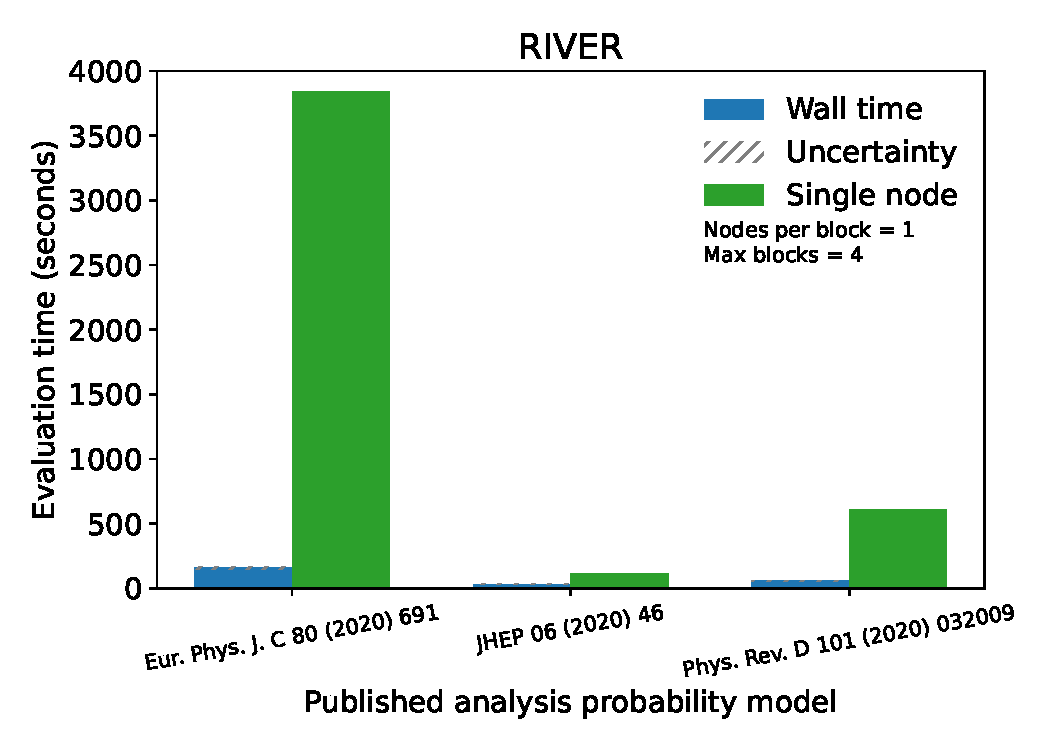
\includegraphics[width=0.8\textwidth]{timing_barplot_river.pdf}
    \caption{Visualization of comparison of the reported wall times in~\Cref{table:performance} categorized by analysis probability model for fits distributed across nodes compared to a single node.}
    \label{fig:timing_barplot_river}
\end{figure}


These results are not fundamental limits of the performance of the software and are meant as preliminary tests of scaling on heterogeneous architecture.
For comparison, on a local system with an AMD Ryzen 9 3900X processor (12 cores 3.8GHz) and 2 x 32GB DDR4-2400 Memory (64 GB) the fitting results for the 125 signal patches of Ref.~\cite{ATLAS_SUSY_1Lbb_pallet} on a single core were obtained in 1672~seconds.
Additionally, in isolated tests on RIVER the 125 signal patches of Ref.~\cite{ATLAS_SUSY_1Lbb_pallet} were able to be fit with \funcX{} orchestration in 76~seconds.
These hardware and block scaling results are parts of ongoing studies to profile the scaling performance of \funcX{} and \pyhf{} for benchmark physics analyses on additional hardware architectures at target HPC facilities.
